
It is of primary interest to apply the \gls{qmla} algorithm to real-life, experimental systems. 
In this chapter we devise an \gls{es} to operate in conjunction with experimental data 
    in order to characterise an electron spin in a \gls{nvc} in diamond.
In particular, we model, through \gls{hamiltonian} terms, interactions between the spin and 
    the spin bath in which it resides,
    so that \gls{qmla} is finding an effective model for the open system dynamics.
\par

Here we will first introduce a basic picture of \glspl{nvc}, 
    using basic but nonstandard nomenclature for simplicity;
    for thorough descriptions of the underlying physics, readers are referred to \cite{doherty2013nitrogen}.
We next discuss the target system with respect to its modelling, 
    determining the suitable terms which \emph{might} represent the \gls{nvc}'s interactions, 
    to inform the starting point for \gls{qmla}.
Finally we describe the implementation of an \gls{es} for the examination of the \gls{nvc},
    and the results of the \gls{qmla} procedure. 

\section{Nitrogen-vacancy centre}
\label{sec:nv_centres}

Nitrogen vacancies are point defects in diamond, 
    occuring intrinsically (naturally) \cite{davies1976optical} or extrinsically (synthetically) \cite{meijer2005generation, edmonds2012production}.
A substitutional \gls{nitrogen} isotope is embedded in a lattice of carbon atoms in diamond, 
    adjacent to a lattice vacancy, 
    such that it is surrounded by three \glspl{carbon} (either $^{12}C$ or $^{13}C$) \cite{lenef1996electronic}. 
Of the \gls{nitrogen} atom's five valence electrons, three bond with nearby \glspl{carbon};
    the remaining two unbonded electrons couple with the lattice vacancy, 
    forming a triplet state, considered as the \gls{nvc}. 
We can experimentally drive the outer electron, moving the \gls{nvc} between energy levels characterised by the triplet. 
In this section we describe how we can exploit those energy levels in order to define a mechanism by which to 
    prepare and implement gates on the controlled system, a readout procedure and a computational basis.

\par 

A \emph{manifold} is a set of states with marginal differences, such as a single differing quantum number.
For example, states near the absolute ground state might differ only in their magnetic spin quantum number:
    together they can be characterised as the \emph{ground state manifold}. 
We consider two principal manifolds of the system:
    the ground state and excited manifolds, each consisting of 
    three states, corresponding to the allowed values for magnetic spin $m_s$, see \cref{fig:nv_centre_energy_levels}a. 
For brevity, we denote states with reference to their magnetic spin and manifold, 
    e.g. the state in the ground state manifold with $m_s=0$ is denoted $\ket{m_s=0}_g$. 
In the absence of a magnetic field, the states corresponding to $\ket{m_s=\pm1}$ are degenerate, 
    but in the presence of a magnetic field, $B$, they have distinct energy levels, 
    referred to as the Zeeman effect, \cref{fig:nv_centre_energy_levels}b. 
\par 

For the purposes of computation, 
    we choose the ground state and one of the excited states as the two levels of a qubit. 
We designate the states $\ket{m_s=0}_g$ and $\ket{m_s=-1}_g$ as the computational basis states $\ket{0}, \ket{1}$ respectively, 
    such that we have defined a qubit and computational basis, \cref{fig:nv_centre_energy_levels}d.
We also require a reliable mechanism through which we can be confident that our qubit is in a definite state, 
    to serve as the starting point of computation: 
    usually qubits are initialised to $\ket{0}$, 
    so here we aim to prepare the \gls{nvc} in $\ket{m_s=0}_g$.
By shining a laser of \SI{532}{\nano\metre} (green) on the \gls{nvc}, irrespective of which state within the ground state manifold the spin starts, 
    it is excited in to the excited manifold, from which it decays back to the ground state manifold.
The process of this decay can be exploited for the preparation of the \gls{nvc} in $\ket{m_s=0}_g$ 
    and therefore enable initialisation for computation.
That is, when the \gls{nvc} is excited to the $\ket{m_s=0}_e$ level, the dominant decay process is spin-preserving, 
    so after decay it ends in $\ket{m_s=0}_g$. 
On the other hand, if the \gls{nvc} had been excited instead to $\ket{m_s=\pm1}_e$,
    the dominant decay process is through a meta-stable/shelving state, 
    which does not preserve spin, so in this case it also ultimately decays to the $\ket{m_s=0}_g$, \cref{fig:nv_centre_energy_levels}\textbf{(c)}.
Therefore, irrespective of the initial state, 
    by shining the green laser on the \gls{nvc} and exciting it into any of the states in the excited manifold, 
    after decay it is most likely that it has been prepared in $\ket{m_s=0}_g = \ket{0}$, 
    providing a starting point from which to perform computation.
\par 

The difference in energy between our defined computational basis states $\ket{0}$ and $\ket{1}$ is 
    $\approx 2.87 \SI{}{\giga\hertz}$, i.e. it is addressible by \gls{mw} radiation.
Via antenna, we can deliver a \gls{mw} pulse upon the \gls{nvc}, driving the \gls{nvc} between the two levels
    providing an implementation of an \ttt{X}-gate. 
Likewise, having initialised the state to $\ket{0}$, we can perform a $\nicefrac{\pi}{2}$ rotation 
    about the logical $z$-axis, by running the \gls{mw} laser for half the time, 
    resulting in the state $\ket{+}$. 
We can similarly devise \gls{mw} radiation to achieve quantum gates and operations on our \gls{nvc} qubit.
We depict these cycles in \cref{fig:nv_centre_energy_levels}c. 
\par

\begin{figure}[t]
    \begin{center}
        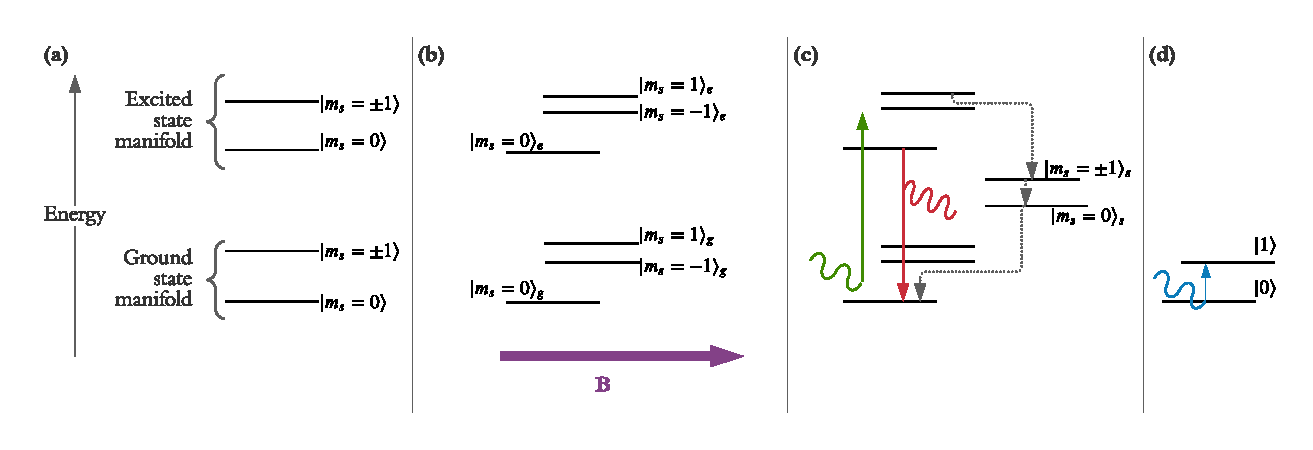
\includegraphics[width=0.95\linewidth]{experimental_study/figures/nv_centre_cartoon.pdf}
    \end{center}
    \caption[\Glsentrylong{nvc} energy levels]{
        Simplified depiction of energy levels of the \glsxtrlong{nvc}, corresponding to its triplet state. 
        \textbf{a}, With no external magnetic field, the system has excited and ground-state manifolds, 
            each of which consist of two energy levels depending on the magnetic spin, $m_s$.
        \textbf{b}, In the presence of a magnetic field (purple, $B$), the magnetic spins have distinct energy levels, 
            i.e. Zeeman splitting giving distinct $m_s$. 
        States are denoted by their magnetic spin, $m_s$ and subscripted by their manifold ($e$ for excited and $g$ for ground-state). 
        \textbf{c},  Application of a \SI{532}{\nano\metre} laser (green arrow) excites the \glsxtrlong{nvc} from any of the states in the 
            ground state manifold into the excited manifold. 
        The dominant decay mechanism for the excited states are shown: 
            (i) $\ket{m_s=0}_e \rightarrow \ket{m_s=0}_g$ (\glsxtrlong{pl}, red) through the emission of a photon at \SI{637}{\nano\metre});
            (ii) $\ket{m_s=\pm 1}_e \rightarrow \ket{m_s=0}_g$ (dotted grey lines) via the shelving manifold which allows for non-spin-preserving transition, 
            emitting a photon in the infrared (not shown).
        \textbf{d}, Computational basis states $\ket{0}$ and $\ket{1}$ are assigned to the two lowest energy states.
            The difference in energy between these states is such that a microwave (MW, blue) 
                can drive transition from $\ket{0} \leftrightarrow \ket{1}$.
            MW pulses can also be used to achieve other states apart from the basis states,
                allowing for the implementation of quantum logic gates. 
    }
    \label{fig:nv_centre_energy_levels}
\end{figure}


We can further exploit the decay mechanism to compose a readout procedure, 
    to infer the population of $\{\ket{0}, \ket{1}\}$ at a given instant, 
    for example following the application of a series of gates (a circuit) to the system. 
We know that the excitation due to the green laser is spin-preserving, 
    i.e. when the \gls{nvc} has been excited to $\ket{m_s=0}_e$, 
    it had originated in $\ket{m_s=0}_g$.
We also know that the decay $\ket{m_s=0}_e \rightarrow \ket{m_s=0}_g$ is spin preserving, with the emission of 
    a red photon: by simply counting the number of excess\footnotemark \ photons emitted, 
    we quantify the population of $\ket{0}$ at the time of query. 
On the contrary, when the $\ket{m_s=-1}_g$ is excited, 
    spin is also preserved, so it goes to $\ket{m_s=-1}_e$, 
    but $\ket{m_s=-1}_e$ decays through the shelving state as outlined earlier, 
    \emph{without} the emission of a red photon (the decay emits out infrared radiation instead). 
We can hence infer the population of $\ket{m_s=-1}_g$ at the time of query by the fraction of incidents which don't 
    emit a photon \cite{knauer2016photonic}.
That is, say we first calibrate the system by retaining the green laser for some time: 
    after a few $\mu s$, a steady state is achieved where the majority of the time, the triplet is in the computional state $\ket{0} = \ket{m_s=0}_g$. 
Then, excitation from the same laser results in the excitation to $\ket{m_s=0}_e$, 
    which decays back to $\ket{m_s=0}_g$ and emits a photon in the process; 
    by counting the red photons emitted in a certain time window -- equivalently, measuring the \gls{pl} signal -- 
    we benchmark the population of $\ket{0}$ when nothing else has happened as $p_0$. 
Now, when we apply gates (i.e. \gls{mw} pulses) to the \gls{nvc}, 
    we can similarly read out the population of $\ket{0}$ as $p_0^{\prime}$,
    and infer that the likelihood that the \gls{nvc} is found in the initial state $\ket{0}$ is $\nicefrac{p_o^{\prime}}{p_0}$. 
We can use this quantity as the  \gls{likelihood} within \gls{qle}, allowing us to learn from the \gls{nvc},
    as we will discuss in the next sections. 

\footnotetext{
    A large number of photons are emitted by the \gls{nvc} when it is excited by a \SI{532}{\nano\metre} laser,
    which can be profiled by its emission spectrum. 
    At the \emph{zero phonon line} (\SI{637}{\nano\meter}),
    a relatively large number of photons are emitted, compared with nearby wavelengths.
    This is where decay from the excited to ground state occurs without interacting with proximal phonons, 
        as is the case during the spin-preserving decay $\ket{m_s=0}_e \rightarrow \ket{m_s=0}_g$.
    The excess photons are taken as indication that the electron had been in the state $\ket{m_s=0}_e$ immediately prior to emission.
}
\par 

In summary then, by assigning computational basis states $\ket{0}, \ket{1}$ to energy levels of the ground state manifold, 
    we are able to ensure the preparation of the \gls{nvc} in $\ket{0}$ by first shining a green laser on the \gls{nvc}. 
We can then apply \gls{mw} radiation to achieve quantum logical gates on the system, 
    and read out the final state of the system, again by shining a green laser
    and observing the \gls{pl} (i.e. the emitted photons), and inferring the population level of each basis state. 
We represent these concepts in a simplified format in \cref{fig:nv_centre_energy_levels}. 

\subsection{Experimental procedure}\label{sec:experimental_procedure}
\begin{figure}
    \begin{center}
        \subfloat[]{
            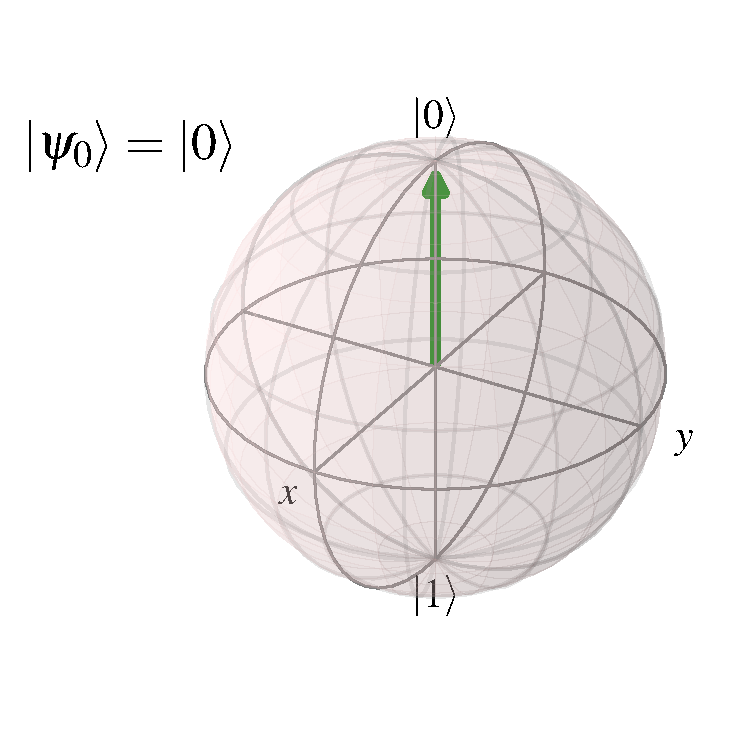
\includegraphics[width=0.25\textwidth]{experimental_study/figures/hahn_bloch_spheres/bloch_0.pdf}
        }
        \qquad
        \subfloat[]{
            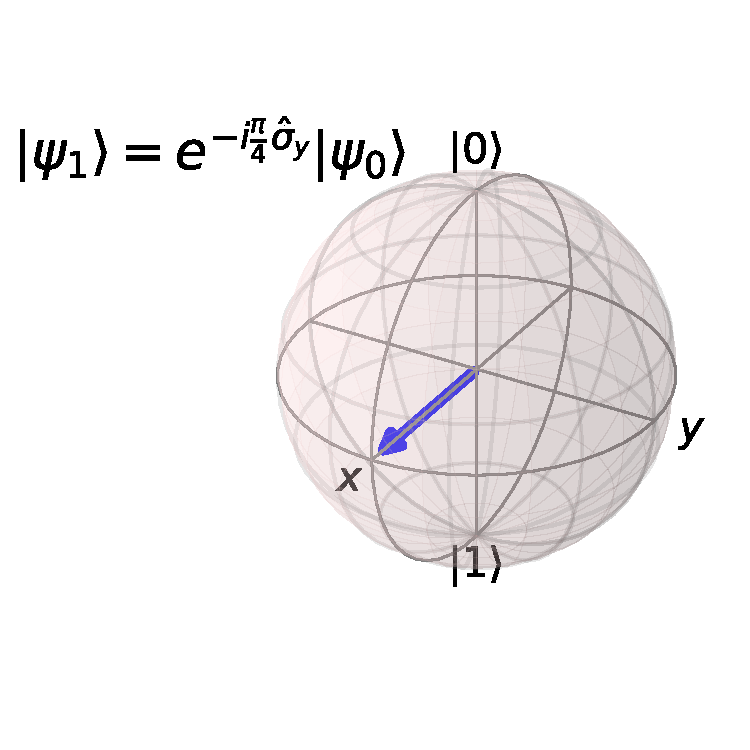
\includegraphics[width=0.25\textwidth]{experimental_study/figures/hahn_bloch_spheres/bloch_1.pdf}
        }
        \qquad
        \subfloat[]{
            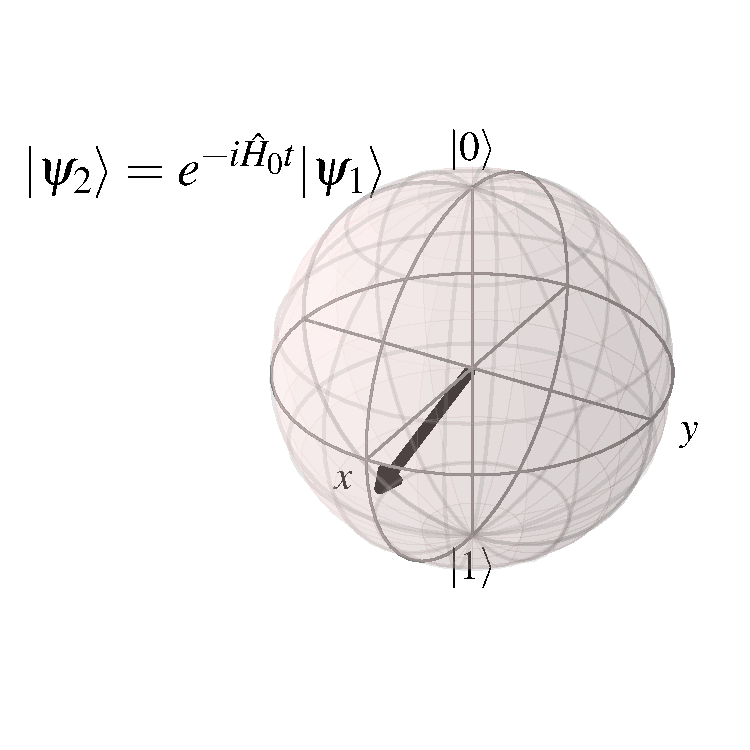
\includegraphics[width=0.25\textwidth]{experimental_study/figures/hahn_bloch_spheres/bloch_2.pdf}
        }
        \\
        \qquad
        \subfloat[]{
            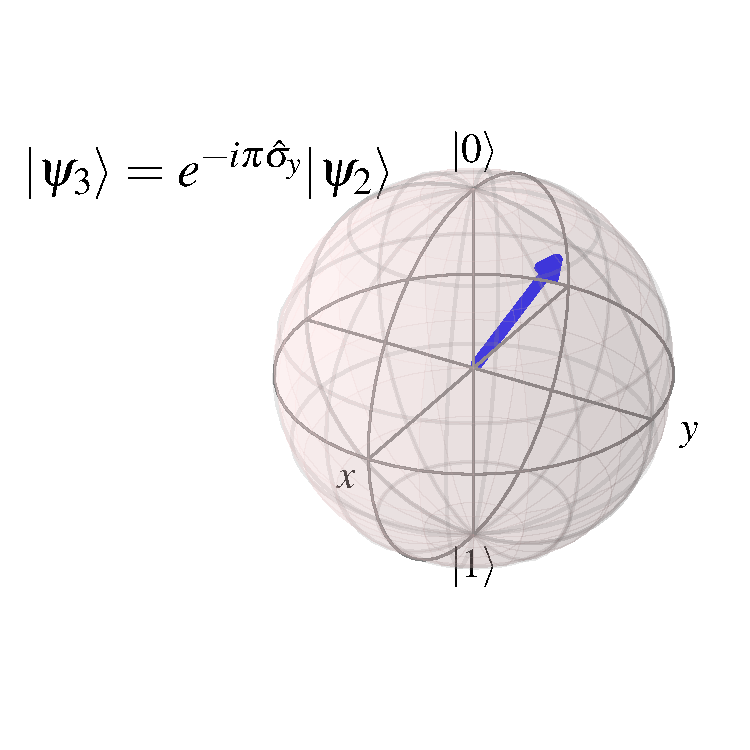
\includegraphics[width=0.25\textwidth]{experimental_study/figures/hahn_bloch_spheres/bloch_3.pdf}
        }
        \qquad
        \subfloat[]{
            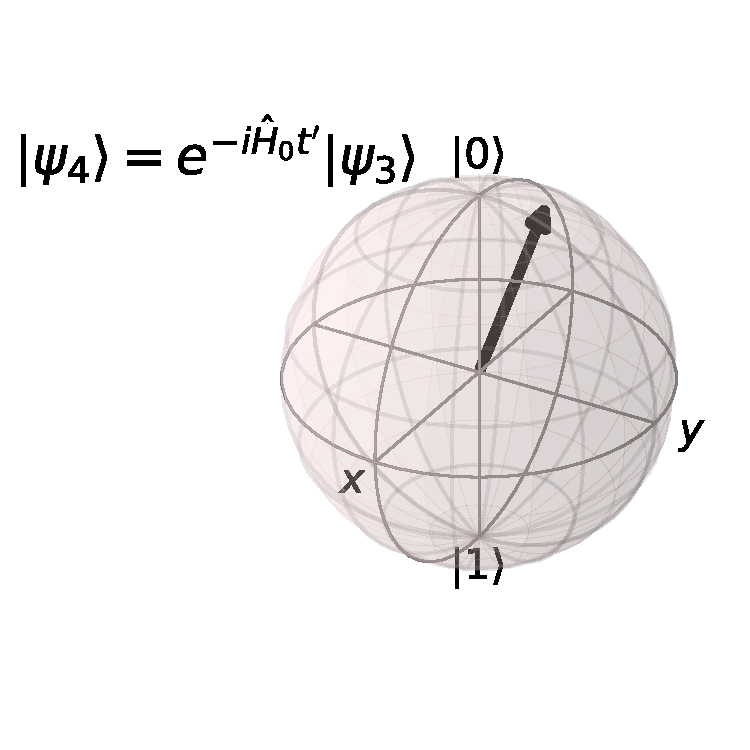
\includegraphics[width=0.25\textwidth]{experimental_study/figures/hahn_bloch_spheres/bloch_4.pdf}
        }
        \qquad
        \subfloat[]{
            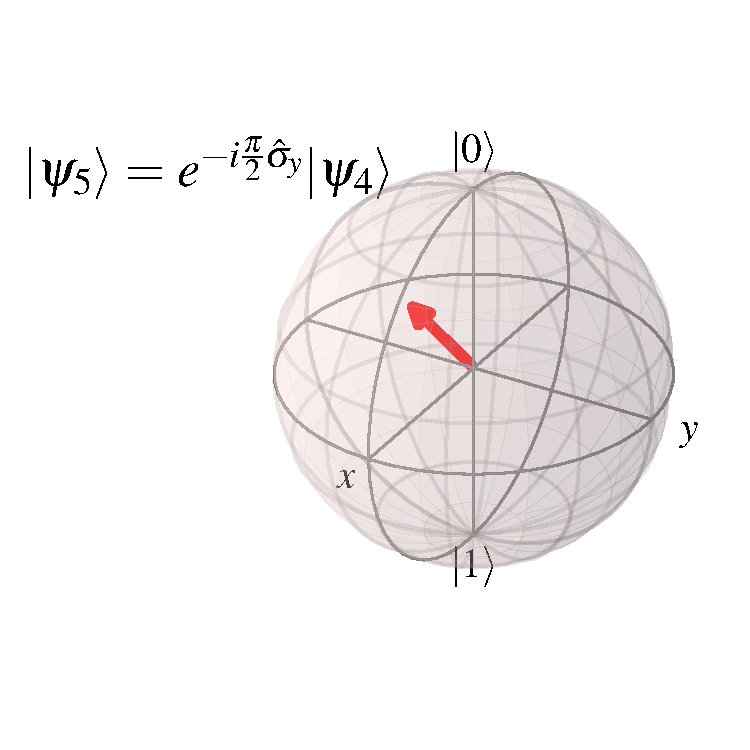
\includegraphics[width=0.25\textwidth]{experimental_study/figures/hahn_bloch_spheres/bloch_5.pdf}
        }
    \end{center}
    \caption[States of spin qubit at each stage of Hahn echo sequence shown on the Bloch sphere]{
        States of spin qubit at each stage of Hahn echo sequence shown on the Bloch sphere.
        \textbf{a,} The state of the \gls{nvc} spin is initialised by a green laser into state $\ket{\psi_0} = \ket{0}$. 
        \textbf{b,} We apply a $\nicefrac{\pi}{2}$ rotation about the $y$-axis (i.e. a \glsxtrfull+{mw} pulse, implemented as $e^{-i \frac{\pi}{4} \s_y}$), 
            yielding the state $\ket{\psi_1} = \ket{+}$. 
        \textbf{c,} The system is allowed to evolve according to its own $\ho$ for $t$, $\ket{\psi_2} = e^{-i\ho t}\ket{+}$.
        \textbf{d,} We apply a second \gls{mw} pulse, this time for a $\pi$-rotation about the $y$-axis, 
        $\ket{\psi_3} = e^{-i\frac{\pi}{2} \s_y}e^{-i\ho t}\ket{+}$.
        \textbf{e,} Again the system evolves according to interactions with the environment, this time for $t^{\prime}$.
        \textbf{f,} We apply a final $\nicefrac{\pi}{2}$ \gls{mw} pulse to rotate about the $y$-axis again, 
            projecting it upon $\ket{0}$.
        Here $\ket{\psi_5}$ is roughly half way between $\ket{0}$ and $\ket{+}$, 
        i.e. along the $z$-axis. 
        The spin is read out from $\ket{\psi_5}$ via the \gls{nvc}'s \glsxtrlong{pl}. 
        Here $\ho = 0.25 \ \s_y$ was evolved for $t=0.5$ (arbitrary units), 
        and the final state overlap with the initial state, 
        i.e. the \gls{likelihood} of measuring the spin in $\ket{0}$ is $\Pr(0 | \ho, t) = 0.865$. 
    }
    \label{fig:hahn_bloch_spheres}
\end{figure}

As our primary objective, we aim to model the decoherence and precession of the \gls{nvc} (described in \cref{sec:target_system}), 
    and therefore must implement an experimental strategy which highlights 
    the decoherence effects dominating the spin. 
The \emph{Hahn echo sequence} is a series of operations which decouple a spin from the  
    slowly varying components of its environment, i.e. the nuclear bath
    \cite{blok2014manipulating, childress2006coherent, rowan1965electron, charnock2001combined, gentile2020Operating}.
For short evolution times, i.e. in the first decay of the \gls{nvc}, the spin is influenced mostly by \emph{fast} decoherence processes,
    providing a platform to study the contributions of dominant decoherence effects in isolation. 


\par 
During the Hahn echo sequence, the \gls{nvc} spin undergoes a series of evolutions -- 
    either according to application of quantum logic gates
    or the natural evolution of the system interacting with its environment.
Intuitively, the stages are as follows: 
\begin{enumerate}[label=(\alph*)]

    \item Prepare spin in $\ket{0}$.
    \item Apply a $\nicefrac{\pi}{2}$ \gls{mw} pulse. 
    A $\pi$-pulse is a \gls{mw} pulse of sufficient duration to flip the spin completely ($\ket{0} \leftrightarrow \ket{1}$), 
    so a $\nicefrac{\pi}{2}$-pulse generates a superposition, i.e. $\nicefrac{\pi}{2}: \ket{0} \rightarrow \ket{+}$.
    \item The superposition precesses freely for $t$. During this time, the $\ket{1}$-component of the superposition picks
        up a phase proportional to $t$, such that the spin is now in the state $\frac{1}{\sqrt{2}}\left( \ket{0} + e^{-i \delta t}\ket{1}\right)$. 
    \item A \gls{mw} $\pi$-pulse is applied, which inverts the basis states, yielding the state $\frac{1}{\sqrt{2}}\left( \ket{1} + e^{-i \delta t}\ket{0}\right)$.
    \item The spin is again allowed precess freely, here for a duration $t^{\prime}$. 
        Again the $\ket{1}$-copmonent gains a phase $e^{-i \delta t^{\prime}}$, 
        i.e. the spin is in the state $\frac{1}{\sqrt{2}}\left( e^{-i \delta t}\ket{0} + e^{-i \delta t^{\prime}}\ket{1} \right)$.
    \item A final $\nicefrac{\pi}{2}$ pulse is applied, giving 
        $\frac{1}{\sqrt{2}}\left( e^{-i \delta t}\ket{+} + e^{-i \delta t^{\prime}}\ket{-} \right)$.
        Expanding $\ket{+}, \ket{-}$ and factoring $e^{-i \delta t}$, we get the final state
        \begin{equation}
            \ket{\psi_H(t, t^{\prime})} = \frac{e^{-i \delta t}}{2} \left\{ (1 + e^{-i \delta(t^{\prime} - t)})\ket{0} + (1 - e^{-i \delta(t^{\prime} - t)})\ket{1}  \right\}.    
        \end{equation}
\end{enumerate}

If the second free evolution is run for $t^{\prime} = t$, we retrieve
\begin{equation}
    \ket{\psi_H(t, t^{\prime}=t)} = \frac{e^{-i \delta t}}{2} \left\{ (1 +1)\ket{0} + (1 - 1)\ket{1}  \right\} = \ket{0},    
\end{equation}
    i.e. the phase accumulated is effectively removed. 
This is therefore an excellent scheme when seeking to isolate the spin from its environment, 
    e.g. when the spin is intended to act as a qubit. 
In practice it is impossible to decouple the environment entirely, 
    since distant nuclei still interact with the spin, % TODO why are these not cancelled out by the same phase reversal?
    causing decoherence on a relatively long time scale\footnotemark.
These are what we refer to as \emph{slow} interactions: 
    this decoupling scheme can therefore be viewed as corresponding to a model 
    where the Hamiltonian consists solely of slow terms, 
    enabling us to study the spin's interactions with its environment beyond 
    the nearest \gls{carbon} atom.
We will explore this possibility in \cref{chapter:many_qubits}.
\footnotetext{
    The timescales on which these interactions decohere the spin are orders of magnitude higher
    then available through alternative decoupling schemes,
    e.g. $T_2 = \SI{242 }{\micro\second}$ in \cite{childress2006coherent}.
}
\par 

On the other hand, when $t^{\prime} \neq t$, the spin is instead found in the state
\begin{equation}
    \label{eqn:hahn_unequal_times}
    \ket{\psi_H(t, t^{\prime}\neq t)} = \frac{e^{-i \delta t}}{2} \left\{ (1 + e^{-i \delta(t^{\prime} - t)})\ket{0} + (1 - e^{-i \delta(t^{\prime} - t)})\ket{1}  \right\}.
\end{equation}

\cref{eqn:hahn_unequal_times} has the precise form (up to the phase factor $e^{-i \delta t}$)
    of a spin having undergone a \emph{Ramsey sequence}, 
    i.e. a $\nicefrac{\pi}{2}$ pulse, followed by free evolution for $t$, and a final $\nicefrac{\pi}{2}$ pulse.
That is, for $t^{\prime}\neq t$, the Hahn echo sequence behaves like 
    a Ramsey sequence with a delay $(t^{\prime} - t)$ \cite{childress2007coherent}. 
$\ket{\psi_H(t, t^{\prime}\neq t)}$ therefore does \emph{not} decouple the spin from its dominant dephasing contributions, 
    but rather it reverses the dephasing due to \emph{slowly varying} components of the environment. 
As such, this provides a platform for examining only the \emph{fast} effects on the spin, 
    i.e. the dominant Markovian decoherence processes, which are expected to be dominated by 
    coupling with the nearest \gls{carbon} atom of strength $\mathcal{O}(\SI{}{\mega\hertz})$. 
\par 

In \cref{chapter:many_qubits}, we consider the system more broadly, and endeavour to 
    characterise its coupling with several nuclei, located farther from the spin than the nearest \gls{carbon},
    i.e. the slower-varying contributions to the spin's dynamics, 
    which an be examined via the former scheme with $t^{\prime} = t$. 
For the remainder of this chapter, however, we will exploit the latter scheme, \cref{eqn:hahn_unequal_times}, 
    in order to model the decoherence of the spin via its relationship with a single \gls{carbon} atom. 
\par 

To relate the experimental procedure to the parameter learning technique described in \cref{chapter:qhl}
    which fulfils the training stage of \gls{qmla}, consider the overal Hahn echo sequence.
We depict the stages of the experiment more generally in \cref{fig:hahn_bloch_spheres}, 
    starting from the initialised computational state, $\ket{\psi_0} = \ket{0}$,
    through to its final state which is read out through \gls{pl},
    both of which as described in \cref{sec:nv_centres}.
In particular, the final state, $\ket{\psi}_5$, is effectively read out by projection onto $\ket{0}$;
    we can interpret the normalised \gls{pl} after evolution time $t$ as the  \gls{likelihood} 
    that the \gls{nvc} is found in $\ket{0}$ after evolution of its \emph{true}\footnotemark \ Hamiltonian, $\ho$ for $t$. 
\footnotetext{
    Note: we refer to the target $\ho$ as the system's \emph{true} Hamiltonian. 
    This is a matter of convention: 
        here $\ho$ is not the Hamiltonian of the complete \gls{nvc} system/environment, 
        but captures only the precession and fast decoherence processes, 
        i.e. $\ho$ is simply the name assigned to the Hamiltonian which models the interactions we aim to uncover. 
}
That is, we assign this projection as the quantity $\Pr(0 | \ho, t)$ (the  \gls{likelihood}), 
    and it can be used within \gls{likelihood} estimation in order to refine a candidate model $\hj$, 
    effectively\footnotemark \ by changing the structure of 
    $\hj$ until $\Pr(0 | \ho, t) \approx \Pr(0 | \hj, t) \ \forall t$. 

\footnotetext{
    Of course this is a gross simplification of \gls{qhl} which is described fully in \cref{chapter:qhl}
}
\par 

By varying the evolution time, $t$, used within the Hahn echo sequence, we can map the \gls{likelihood} against time, 
    which we can view as capturing the \emph{dynamics} of the \gls{nvc} spin, \cref{fig:nv_raw_data}.
We vary the evolution time up to $t {\sim} 4 \mu s$ in intervals of $\Delta t = 50 \SI{}{\nano\second}$, 
    so we have 425 data points. 
Note the data for the studied \gls{nvc} is taken once and analysed offline, 
    i.e. \gls{qmla} does not have complete authority to design \glspl{experiment} 
    to run on the \gls{nvc}, although it can aim to choose the most informative $t$ 
    available in the predefined set; we will discuss the consequences of this restriction 
    in \cref{sec:nv_constraints}. 

\begin{figure}[t]
    \begin{center}
        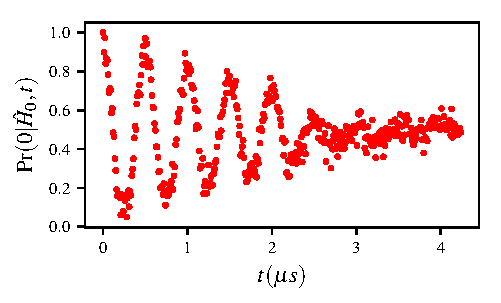
\includegraphics{experimental_study/figures/raw_data.pdf}
    \end{center}
    \caption[Raw data for nitrogen-vacancy centre's dynamics]{
        Raw data for the \glsxtrlong{nvc}'s dynamics.
        The $y$-axis shows the normalised \glsxtrlong{pl} of the \gls{nvc}, 
        equivalently the \gls{likelihood} $\Pr(0 | \ho, t)$. 
    }
    \label{fig:nv_raw_data}
\end{figure}

\section{Target system}\label{sec:target_system}
We take the axis of the \gls{nvc}, i.e. the axis connecting the \gls{nitrogen} with the 
    lattice vacancy, as the $z$-axis.
While the \gls{nvc} is subject to myriad interactions which result in decoherence,
    we choose to focus on its dominant interactions with proximal environmental nuclei. 
These interactions are characterised by hyperfine terms \cite{smeltzer201113c}.
The complete \gls{hamiltonian} for such systems, where the set of nuclear sites is $\{\chi\}$,
    is expected to be given by 

\begin{equation}
    \label{eqn:nv_ham_full}
    \hat{H}_{\mathrm{\textrm{full}}} 
    = 
    \Delta_{\textrm{gs}} \hat{S}_z^2 
    + \mu_B g \mathbf{B} \cdot \mathbf{S} 
    + \mathbf{S} \cdot \sum_{\chi} \left( \mathbf{A}_{\chi} \cdot \hat{I}_{\chi} \right) 
    + P \hat{I}_z^2 
    + \mu_n g \mathbf{B} \cdot \sum_{ \chi} \hat{I}_{\chi}.
\end{equation}

Our overarching intention is to design an approximate model $\hp$, 
    i.e. a subset of the terms in $\hat{H}_{\textrm{full}}$ which can explain the observed dynamics 
    and decoherence of the \gls{nvc}. 
It is therefore prudent only to retain terms which \emph{may} contribute to the spin's decoherence and precession. 
First, we will describe each term in \cref{eqn:nv_ham_full}, 
    as well as approximations which enable us to drastically reduce the space of terms to consider for inclusion in $\hp$. 

\begin{description}
    \item[Isolated-spin terms] \
    
    Describe the spin independent of the environmental nuclei.
    \begin{easylist}[itemize]
    && $\Delta_{\textrm{gs}} \hat{S}_z^2$: 
        the \emph{zero-field} splitting, or ground state splitting between the computational basis states.
        $\Delta_{\textrm{gs}} {\sim} \mathcal{O}(\SI{}{\giga\hertz})$ is a constant offset which does not contribute to the decoherence, 
        so it is excluded from our study.

    && $\mu_B g \mathbf{B} \cdot \mathbf{S}$: 
        the spin's precession about the magnetic field, 
        $\mathbf{B} = \left(B_x \  B_y \  B_z\right)$, 
        via the total spin operator\footnotemark \ $\mathbf{S} = \left(\hat{S}_x \ \hat{S}_y \ \hat{S}_z \right)$, 
        where $\mu_B$ is the Bohr magneton and $g$ is the electron $g$-factor 
        ($\approx 2$, simplified from the $g$-factor tensor).
        Misalignment of the magnetic field is a decoherence effect, 
        so one core aim of \gls{qmla} in this setting is to identify whether such terms dominate.
    \end{easylist}
    
    \item[Hyperfine terms] \ 
    \begin{easylist}
    && $\hat{S} \cdot \sum_{\chi} \left( \mathbf{A}_{\chi} \cdot \hat{I}_{\chi} \right)$:
        The \gls{nvc} total spin operator $\mathbf{S}$ couples the spin with each site, $\chi$.
        At each site there is a nucleus which has total spin operator 
        $\mathbf{I}_{\chi} = \left(\hat{I}_x \ \hat{I}_y \ \hat{I}_z \right)_{\chi}$. 
        $\mathbf{A}$ is the hyperfine tensor, containing the hyperfine parameters of interest. 
        The coupling between the \gls{nvc} and these nuceli is one of the primary decoherence mechanisms, 
        so is essential to any model aiming to capture those dynamics. 
    \end{easylist}

    \item[Bath-only terms] \
    
    Describe the other nuceli independent of the spin
    \begin{easylist}        
    && $P \hat{I}_z^2 $: the quadrupole splitting, which provides another constant shift, 
        and is therefore not of interest when modelling the spin's decoherence, and can be neglected.
    && $\mu_n g \mathbf{B} \cdot \sum_{ \chi} \hat{I}_{\chi}$:
        nuclear precession terms. 
        $\mu_n$ is the nuclear magneton and $g$ is the nuclear $g$-factor (again from the $g$-factor tensor).
        These terms represent the nuclei independent of the spin -- 
        these terms lead to decoherence at much higher times than we have access to, 
        since the Hahn echo sequence reverses the contribution on the spin from the bath, 
        \cref{sec:experimental_procedure}. 
        For the short-time model targeted here, then, these terms can be excluded. 
    \end{easylist}

\end{description}

\footnotetext{
    We invoke an inexact representation of high dimensional tensors here for ease of interpretation. 
    For instance, the total nuclear spin operator exists in arbitrary dimension 
    (depending on the number of sites modelled), 
    but we present it simply as $\mathbf{I} = \left( \hat{I}_x \ \hat{I}_y  \ \hat{I}_z \right)$ at each site 
    to convey that we can separate the terms in the construction of models. 
}

Given that we are modelling the spin's decoherence, 
    we are interested only in the spin and its interactions with the environment, 
    so we can immediately drop the bath-only terms, 
    by assuming the bath is static apart from its interactions with the \gls{nvc}. 
This is a usual assumption in the treatment of open system dynamics, 
    to allow for focus on the dominant interactions in the processes of interest \cite{breuer2002theory}. 
Additionally, since the zero field splitting contributes a constant shift in energy, 
    we can safely omit it by moving to the rotating frame. 
We are then left only with the second and third terms of \cref{eqn:nv_ham_full}, 
    from which to define the space of terms in which \gls{qmla} will search:

\begin{subequations}
    \begin{equation}
        \label{eqn:nv_spin_terms}
        \mu_B g \mathbf{B} \cdot \mathbf{S};
    \end{equation}
    \begin{equation}
        \label{eqn:nv_hyperfine_terms}
        \mathbf{S} \cdot \sum_{\chi} \left( \mathbf{A}_{\chi} \cdot \mathbf{\hat{I}}_{\chi} \right).
    \end{equation}
\end{subequations}

\subsection{Mapping to model terms}
Next we will focus on mapping the remaining terms to operators to compose the set of terms 
    $\termset$ to use in our \gls{es}. 
In our modelling, the \gls{nvc} spin is represented by the first logical qubit, 
    with a further $|\{\chi\}|$ qubits, each representing a unique nuclear site, 
    as discussed later in this section. 
As standard, we take the axis\footnotemark \ of the \gls{nvc} as parallel to the qubit's $z$-axis. 

\footnotetext{The quantisation axis, i.e. the axis along the \gls{nitrogen} and lattice vacancy.}
\par 

The first terms included, \cref{eqn:nv_spin_terms}, come from the spin's precession about the magnetic field. 
It is usually assumed that the external, applied magnetic field is well-aligned with the spin qubit's $z$-axis:
    if the field is misaligned, it leads to decoherence effects. 
Determining the alignment is treated as a core role of \gls{qmla}, 
    i.e. we will endeavour to establish whether the $x$-, $y$-axis components of the magnetic field 
    are important for describing the spin's decoherence. 
Then, we have
\begin{equation}
    \label{eqn:spin_tensor_terms}
    \mu_B g \mathbf{B} \cdot \mathbf{S} 
    = \mu_B g \irow{B_x & B_y & B_z} \cdot \irow{\hat{S}_x & \hat{S}_y & \hat{S}_z}
    \rightarrow \alpha_x \hat{S}_x + \alpha_y \hat{S}_y + \alpha_z \hat{S}_z,
\end{equation}
with $\alpha_i = \mu_B g B_i$. 
The spin's rotation terms to be included in \gls{qmla}'s deliberations are therefore 
\begin{equation}
    \label{eqn:exp_spin_terms}
    \termset_{s} = \{ \hat{S}_x, \  \ \hat{S}_y, \ \ \hat{S}_z\}.
\end{equation}
\par 

Next, we consider the hyperfine coupling term. 
In general we sum over the nuclear sites $\{ \chi \}$, 
    since  the \gls{nvc} spin will interact with every nucleus within a certain range.
We show in \cite{gentile2020learning} that a realistic system requires modelling a 
    finite-size bath of $|\{\chi\}|{\sim}15$ 
    nuclei to capture the dynamics of interest, 
    which is infeasible for complete characterisation via classical simulation, 
    where we are limited to ${\sim}11$ qubit calculations\footnotemark. 
Instead, by focusing only on the \emph{short-time} dynamics of the \gls{nvc}, 
    we can isolate the effects of dominant interactions, 
    most notably with a single nearby \gls{carbon}. 
Indeed, by assigning a first qubit as representing the \gls{nvc} spin, 
    we can map the entire environment onto a generic second \emph{environmental qubit}, 
    representing the amalgamation of said interactions, 
    though we can think of the two-qubit system as the \gls{nvc} coupled with a single \gls{nitrogen} \cite{smeltzer201113c}. 

\begin{equation}
    \mathbf{S} \cdot \sum_{\chi} \left( \mathbf{A}_{\chi} \cdot \mathbf{I}_{\chi} \right)
    \rightarrow 
    \mathbf{S} \cdot \mathbf{A} \cdot \mathbf{I} 
\end{equation}

This reduces the dimension of our approximation: 
    the number of qubits required, $n_q$ 
    reduces from $n_q = 1 + |\{\chi\}|$ to $n_q = 2$, 
    since now we only retain qubits for the \gls{nvc} and the \gls{nitrogen} 
    (which also represents the entire bath).
The hyperfine tensor $\mathbf{A}$ consists of the hyperfine parameters, 
    i.e. the strength of correspdoning interactions. 
\begin{equation}
    \mathbf{A} = 
    \begin{pmatrix}
        A_{\perp} & 0 & 0 \\    
        0 & A_{\perp} & 0 \\
        0 & 0 & A_{\|} \\
    \end{pmatrix},
\end{equation}
    where $A_{\perp}$ is the non-axial hyperfine coupling term and $A_{\|}$ is the axial coupling term, 
    since the axis of the \gls{nvc} is used to define the $z$-axis for our qubits. 

The total spin operators are then those of the \gls{nvc} operating on the first logical qubit, e.g. $\hat{S}^{(1)}_x$,
    and those of the environmental qubit on the second, e.g. $\hat{I}_x^{(2)}$. 
They can be summarised as
\begin{equation}
    \label{total_spin_operators}
    \begin{split}
    \mathbf{S} = \irow{ \hat{S}_x^{(1)}  & \hat{S}_y^{(1)} & \hat{S}_z^{(1)} } \\
    \mathbf{I} = \irow{ \I_x^{(2)} & \I_y^{(2)} & \I_z^{(2)}  } 
    \end{split}
\end{equation}

So we can write, 
\begin{equation}
    \begin{split}
        \mathbf{S} \cdot \mathbf{A} \cdot \mathbf{I} 
        = &A_{\perp} \hat{S}_x \I_x + A_{\perp} \hat{S}_y \I_y + A_{\|} \hat{S}_y \I_y \\
        &+ A_{xy} \left( \hat{S}_x \I_y + \hat{S}_y \I_x \right) \\
        &+ A_{xz} \left( \hat{S}_x \I_z + \hat{S}_z \I_x \right) \\
        &+ A_{yz} \left( \hat{S}_y \I_z + \hat{S}_z \I_y \right) \\
    \end{split}
\end{equation}

Similarly to $\alpha_i$ in \cref{eqn:spin_tensor_terms}, we replace the expected (and theoretically computable)
    scalar parameters, e.g. $A_{\perp}$, with generic parameters $\alpha$, to be learned.
Off-diagonal terms, referred to hereafter as \emph{transverse} terms ($\hat{S_i}\I_j$ where $i\neq j$),
    are usually neglected \cite{blok2014manipulating}.
Here we will employ \gls{qmla} to determine whether the transverse contributions are worthy of inclusion in the decoherence model, 
    although we consider only $\{ \hat{S}_x\I_y, \hat{S}_x\I_z, \hat{S}_y\I_z\}$ for brevity. 
The hyperfine terms to be entertained by \gls{qmla} are then

\begin{equation}
    \termset_{HF} = \left\{
    \begin{align}  
        \begin{split}
        & \hat{S}_x\I_x, && \hat{S}_y\I_y, && \hat{S}_z\I_z, \\
        & \hat{S}_x\I_y, && \hat{S}_x\I_z, && \hat{S}_y\I_z 
        \end{split}
    \end{align}
    \right\}.
    \label{eqn:exp_hf_terms}
\end{equation}

\footnotetext{
    This limitation arises from the requirement to compute the total evolution of the global state, 
    involving calculation of $e^{-i\h t}$, i.e. the characterisation of an $n_q$-qubit model depends on 
    classical exponentiation of the $2^{n_q} \times 2^{n_q}$ \gls{hamiltonian} for each \gls{particle} and experiment in \gls{cle}, 
    which is prohibitively expense. 
}
\par 

Finally, combining \cref{eqn:exp_spin_terms} and \cref{eqn:exp_hf_terms}, 
    we have the full set of terms to incorporate into the \gls{es} for the \gls{qmla} \gls{model search}: 

\begin{equation}
    \termset_{\textrm{NV}} = \left\{
    \begin{align}
        & \hat{S}_x, && \hat{S}_y, && \hat{S}_z, \\
        & \hat{S}_x\I_x, && \hat{S}_y\I_y, && \hat{S}_z\I_z, \\
        & \hat{S}_x\I_y, && \hat{S}_x\I_z, && \hat{S}_y\I_z 
    \end{align}
    \right\}.
    \label{eqn:nv_terms_verbose}
\end{equation}
\par 

We introduce a shorthand notation to ease model representation for the remainder of this chapter. 
Recall that we have defined a two-qubit Hilbert space for model construction.
Terms which affect only the spin act only on the first qubit, $\hat{S}_i = \hat{S}_i^{(1)} = \s_i \otimes \ident$, 
    where $\s_i$ is the Pauli operator giving rotation about the $i$-axis, and 
    $\ident$ is the one-qubit identity matrix. 
Retaining the hyperfine notation, for the expectedly-dominant diagonal terms, we denote $\hat{A}_i = \hat{S}_i^{(1)} \I_i^{(2)} = \s_i \otimes \s_i$. 
We refer to the transverse terms as $\hat{T}_{kl} = \hat{S}_k^{(1)} \I_l^{2} = \s_k \otimes \s_l$. 
We can hence rewrite \cref{eqn:nv_terms_verbose} as 
\begin{equation}
    \label{eqn:nv_terms}
    \termset_{\textrm{NV}} = \left\{ 
        \begin{split}    
            &\hat{S}_x, && \hat{S}_y,  && \hat{S}_z, \\
            &\hat{A}_x,  && \hat{A}_y,  && \hat{A}_z, \\
            &\hat{T}_{xy},  && \hat{T}_{xz}, && \hat{T}_{yz} 
        \end{split}
    \right\}.
\end{equation}

We also use a succinct representation for brevity, e.g. $\hat{S}_{xy}\hat{A}_z =  \hat{S}_x + \hat{S}_y + \hat{A}_z$, 
    where parameters $\alpha_x, \alpha_y, \alpha_z$ are implicitly assumed. 

\subsection{Prior knowledge}

\gls{qmla} will construct models using the pool of terms defined in \cref{eqn:nv_terms}. 
Recall from \cref{chapter:qmla} that each model considered must be trained independently, 
    where the purpose of model training is to optimise the parameter vector $\al$ which characterises the model. 
For example, the model 
    $\hi = \hat{S}_{x,y} \hat{A}_{z} = \alpha_1 \hat{S}_x  + \alpha_2 \hat{S}_y + \alpha_3 \hat{A}_z$,
    is trained to retrieve the optimal $\al^{\prime}_i = \irow{\alpha_1^{\prime} & \alpha_2^{\prime} & \alpha_3^{\prime}}$. 
Models are trained through \gls{qhl}, described in \cref{chapter:qhl}, 
    which iteratively updates a probability distribution for the associated parameters, $\Pr(\al)$. 
As such, a \emph{prior} distribution must be drawn, from which \gls{qhl} begins its training. 
While \gls{qhl} can redraw the probability distribution iteratively, and even find parameters entirely outside of the initial range, 
    it is necessary at least to identify the order of magnitude where the true parameter should be found. 
The algorithm therefore demands that the user specifies the \emph{range} of each parameter in which to search, 
    which can be based on domain knowledge and theoretical predictions. 
For example, recall from \cref{sec:target_system} that the zero field splitting, $\Delta_{gs}$ in \cref{eqn:nv_ham_full} (and excluded in our modelling),
    is expected to be $\mathcal{O}\left( \SI{}{\giga\hertz}\right)$: in order to provide a reasonable chance at learning the true parameter,
    here we would propose a prior distribution of $5 \pm 2 \SI{}{\giga\hertz}$.
We must similarly identify the broad range in which we reasonably expect to find parameters associated with each term in \cref{eqn:nv_terms}.
\par

The spin-only terms, $\hat{S}_i$, are consequences of the magnetic field, 
    expected in the range $\mathcal{O}\left(2-3\SI{}{\mega\hertz}\right)$.
Likewise, the hyperfine terms, $\hat{A}_i$ are expected in the range of $\mathcal{O}\left( \SI{}{\mega\hertz}\right)$ \cite{gali2008ab}, 
    while in the \emph{secular approximation} only the $z$-component is expected to contribute substantially \cite{dutt2007quantum}. 
The non-axial hyperfine terms, i.e. the transverse terms $\hat{T}_{kl}$ are not usually included in effective models, 
    but can be found of order $\mathcal{O}(\SI{10}{\kilo\hertz})$ \cite{hou2019experimental}. 
We utilise this prior understanding of the system to inform the parameter range used for training candidate models:
    for each of the terms in \cref{eqn:nv_terms}, we will adopt a normal prior distribution of $4 \pm 1.5\SI{}{\mega\hertz}$. 
This range is sufficiently specific to ensure the training subroutine operates in a physically meaningful -- 
    and likely appropriate -- space, while also broad enough to allow for significant differences between expectation and reality.
Moreover this distribution supports hypotheses where each parameter is zero:
    if these prove favourable, negligible contributions can be identified and excluded from the model.

\section{Exploration strategy}\label{sec:exp_es}
We may now turn to the specific implementation details by which \gls{qmla} is applied to the study of this \gls{nvc} system. 
Recalling the terminology of \gls{qmla} from \cref{chapter:qmla}, 
    we design an \acrfull{es} specifically for the system under study. 
The \gls{es} will account for the details listed in this chapter so far, in summary: 
\begin{easylist}[itemize]
    & we aim to assign a model, $\hp$, to the \gls{nvc} to describe its decoherence processes
    && we especially focus on its hyperfine interactions;
    & we use a 2-qubit approximation
    && the first qubit represents the spin itself;
    && the second qubit represents the environment in which the \gls{nvc} resides;
    & we query the \gls{nvc} by performing Hahn echo \glspl{experiment} (\cref{fig:hahn_bloch_spheres});
    & the outcome of those \glspl{experiment} are thought of as the system's \glspl{likelihood}  (\cref{fig:nv_raw_data});
    & candidate models are composed of the terms defined in \cref{eqn:nv_terms}
    && \glspl{likelihood}  are used for the training of individual candidate models through \gls{qhl};
    && we assign approximate ranges to the scalar parameters corresponding to each term based on theoretical arguments;
    &&& those parameters are to be learned precisely by \gls{qhl}.
\end{easylist}   
\par 

As outlined in \cref{sec:exploration_strategies}, the central role of any \gls{es} is to specify the 
    model generation procedure, which \gls{qmla} relies upon for deciding the next set of candidate models to test. 
In this case, we exploit some intuition and prior knowledge of how such systems work, 
    to design a bespoke model generation subroutine:
    we can think of this as a midway point between the completely specified \glspl{es} used 
    for identifying the underlying lattices from a prescribed set in \cref{chapter:lattices}, 
    and the entirely general \glsxtrlong+{ga} which does not restrict model generation, of \cref{chapter:ga}.
We use the standard structure of \glspl{et} introduced in \cref{sec:exploration_strategies}, 
    where models are placed on consecutive branches, $\mu$, and branches are consolidated by pairwise comparisons between all models on $\mu$, 
    where comparisons are computed through \glspl{bf}.
The outcome of consolidation on $\mu$ is the determination of a single \emph{branch champion}, $\hat{H}_{C(\mu)}$. 
\par 


\begin{figure}
    \begin{center}
        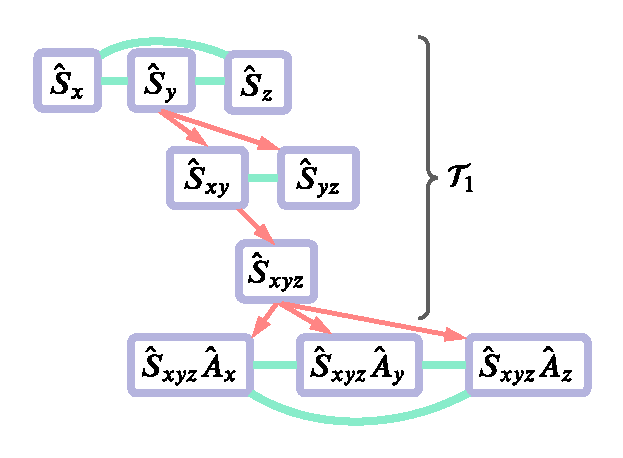
\includegraphics[width=0.5\textwidth]{experimental_study/figures/greedy_search.pdf}
    \end{center}
    \caption[Greedy model search]{
        Greedy \gls{model search}. 
        Models (purple) are placed on branches, trained and consolidated (green) as in \cref{fig:qmla_overview}, 
            with the branch champion spawning (red) candidates to place on the subsequent branch.  
        Branches are grouped in tiers, correspdoning to levels of approximation:
            the first tier of the model generation strategy is shown, 
            where $\termset_1 = \{ \hat{S}_x, \hat{S}_y, \hat{S}_z\}$ is explored. 
        The final champion from the first tier seeds the second tier. 
    }
    \label{fig:greedy_search}
\end{figure}

We use a \emph{greedy search rule}: 
    terms are added one-by-one to gradually increase the complexity of candidate models until terms are exhausted \cite{russell2002artificial}.  
We break the \gls{et} into three distinct tiers, each corresponding to an intuitive degree of complexity:
    the first tier involves the spin-only terms, $\termset_1 = \{ \hat{S}_i \}$; 
    the second considers the hyperfine terms, $\termset_2 = \{ \hat{A}_i \}$;
    the final tier the transverse terms, $\termset_3 = \{ \hat{T}_i\}$.  
Within each tier, terms are added greedily to the previous branch's champion, $\hat{H}_{C(\mu)}$.
So, the first branch is given by $\mu = \{ \hat{S}_x, \hat{S}_y, \hat{S}_z\}$;
    say $\hat{H}_{C(\mu)} = \hat{S}_y$, then $\mu + 1$  determines that $\hat{S}_x, \hat{S}_z$ 
    are not yet considerd, so it constructs the models $\{\hat{S}_{x,y}, \hat{S}_{y,z}\}$, e.g. \cref{fig:greedy_search}. 
After exhausting all tiers, we consolidate the set of branch champions, $\mathbb{H}_C = \{ \h_{C(\mu)}\}$, 
    to determine the best model considered globally, $\hp$.  
\par 

Clearly, this growth rule is partially deterministic, insofar as some models are guaranteed to be considered, 
    while others are not reachable.
Indeed, the space of available models are heavily constrained, in particular models in later tiers will 
    always involve all of the tier 1 terms, e.g. $\hat{S}_{x}\hat{A}_{y}$ can not occur organically. 
In general, restrictions of this kind undermine the \gls{es} and are considered a weakness.
To account for this, we add a final test of reducibility on the \gls{champion model}, 
    triggered if any of the parameters of $\al^{\prime}$ are potentially negligible, 
    i.e. the posterior distribution of any parameter assigns credibility to the hypothesis that the parameter is 0.
This champion reducibility test simply removes the negligible-parmeter terms from $\hp$, 
    yielding a reduced global champion, $\hp_r$.
We then compute the \gls{bf} between $\hp, \hp_r$: 
    if the \gls{bf} indicates strong evidence in favour of the reduced version, 
    we replace the \gls{champion model}, $\hp \gets \hp_r$. 
In effect, we thus verify the statistical significance of each term included in $\hp$. 
\par 

The total model in \cref{eqn:nv_ham_full} supports $N_t = 1 + 3 + 6 | \chi | + 3 + 3 |\chi| = 7 + 9|\chi| $ terms, 
    which we reduced to a space of $N_t=3 + 6 |\chi| = 9$ through several approximations.
Even so, the remainng $2^9$ permitted models were reduced further by building the logic of this \gls{es} 
    from our intuition aroud existing knowledge of typical \gls{nvc} systems.
As such, the described \gls{es} will only ever consider $<20$ models per instance. 
The described \gls{es} seems overly perscriptive, 
    but should be viewed as a first attempt at a generalisable approach: 
    essentially we can view the tiers of the greedy search as characterising the system 
    at various approximations, 
    e.g. the first tier examines one-qubit terms, while subsequent tiers inspect $2$-qubit terms. 
We can envision future work where the greedy search is gradually extended to less rigid approximations, 
    enabling study of more complex quantum systems.     
This leads to some important remarks:

\begin{easylist}[enumerate]
    \ListProperties()
    & Realistic, near-term applications of \gls{qmla} can not be thought of as a solution to black-box characterisation problems: 
        it must be used in conjunction with domain expertise for the system under study.
    & While this test-case yields promising results, the outcome of \gls{qmla} here may not be especially insightful, 
        since the available model terms were so deliberately constrained -- we demonstrate a use-case in \cref{chapter:many_qubits} 
        where a broader scope is enabled in simulation.    
\end{easylist}   
\par 

A common charge against \gls{qmla} supposes to first write down the most complex model, 
    train it fully, and then infer which terms are negligible, in a similar process to the champion reduction test outlined here. 
While this may be feasible in the case described here, with $N_t=9$ and a closed term set, 
    it is unscalable: adding just a second nuclear site increases the \gls{model search} to a space of $N_t=15$.
Models of higher cardinality ($|\al|$) demand higher \gls{nexp}, \gls{nprt} to train well, so immediately training the most involved model would 
    require infeasible resources\footnotemark, and risks significantly overfitting the data. 
It seems more appropriate to work ``from the ground up'', testing terms and only keeping those justified, 
    rather than training all terms and attempting to decouple their effects post-hoc. 

\footnotetext{
    Note: in the case studies presented in this thesis, it was found that the same resources were sufficient for the simplest and most complex models, 
    due to the relatively small number of terms therein.
    We expect for larger models, e.g. $|\al|>10$, that the resources allocated ought to be proportional to the cardinality, 
    which is an in-built option in the \gls{qmla} software. 
}
\par 
\subsection{Test in simulation}
Before considering the real experimental data (\cref{fig:nv_raw_data}), 
    we first test the \gls{es} in simulation under ideal conditions. 
That is, we assume the ability to prepare arbitrary \gls{probe} states, 
    and use a random \gls{probe} set (see \cref{sec:probes}),
    and use the full expectation value as the likelihood, $|\braket{\psi | e^{-i \hj t} | \psi}|^2$.
Of course, this is infeasible since we presume access to the full state at the time of measurement, 
    but this can be seen as a best-case scenario for this application, 
    because the realistic case loses information by tracing out the environmental qubit at measurement.
We vary the target $\ho$, among a series of ten models,
    which are all valid models achievable by the \gls{es}. 


\section{Experiment design constraints}\label{sec:nv_constraints}
Moving to analyse the experimental setup, there are a number of constraints which we must account for in 
    training models. 
Firstly, the $\nicefrac{\pi}{2}$-pulse applied to the prepared qubit ($\ket{\psi_0} \rightarrow \ket{\psi_1}$ in \cref{fig:hahn_bloch_spheres})
    means that the state before evolution is always $\ket{+}$ in the computational basis;
    this is a severe limitation on model training, as we saw in \cref{sec:heuristic}. 
Moreover, this places a bias on the interactions \gls{qmla} is likely to identify:
    we show in \cref{fig:hahn_bloch_spheres} how \gls{qhl} performs in training the same model using 
    (i) the \gls{probe} set available experimentally; (ii) a more general (random) \gls{probe} set. 
This bias adds a caveat to the outcome of this study:
    the suppression of terms means we are more likely to find some genuine interactions than others, 
    so the \gls{champion model} is capturing the decoherence with respect only to one basis.
\par

The experiment was run with increasing $t$ for the duration of the first decay of the \gls{nvc}, 
    i.e. until it had dephased, 
    so the data available for examination terminate at $t_{\textrm{max}} {\sim} 4 \mu s$, see \cref{fig:nv_raw_data}. 
As discussed in \cref{sec:heuristic}, usually it is helpful to allow an \gls{edh} to
    choose the experimental controls, including the evoltuion time, $t$, against which 
    the model is trained at each experiment;
    the default \gls{pgh} attempts to select $t$ at the upper boundary of times 
    where the model is expected to be predictive, to maximise the information gained by the experiment (see \cref{sec:pgh}). 
Here, however, we can not allow the \gls{edh} to select arbitrary $t$, 
    since we do not have data beyond $t_{\textrm{max}}$. 

\par 

We require a custom \gls{edh} to account for the constraints outlined, 
    with the following considerations: 
\begin{easylist}[enumerate]
    & We may only assume access to the \gls{probe} $\ket{+}$ on the spin qubit
    && we further assume the environmental spin is polarised by the same microwave pulse, 
        such that the global \gls{probe} available is $\ket{\psi} = \ket{+}\ket{+^{\prime}}$, with 
        $\ket{+^{\prime}} = \frac{\ket{0} + e^{i \phi} \ket{1}}{\sqrt{2}}$ and $\phi$ is random \cite{broadway2018quantum}. 
    & We can not allow the choice of any $t$:
    && Any $t > t_{\textrm{max}}$, arising from a thin parameter distribution, 
        must be mapped to some $0 < t \leq t_{\textrm{max}}$. 
    && All nominated $t$ must be mapped to the nearest available $t$ in the dataset
        so that the \glspl{likelihood}  are as close as possible to simulating the true system. 
    & Much of the physics of interest occurs at relatively high times, 
        i.e. because the rotation ($\SI{}{\mega\hertz}$) terms dominate, the decay of the peaks
        can be seen as evidence of the bath, notably through hyperfine terms in the model. 
    && We therefore wish to enforce that all models are trained on those data ($t \geq 2 \mu s)$,
        even if their parameter distribution is insufficiently narrow to yield those times naturally. 
\end{easylist}

Accounting for these, we construct an \gls{edh} which mixes the robust, adaptive nature of \gls+{pgh}, 
    useful for refining an initially broad $\Pr(\al)$,
    with a primitive, linear time-selection, useful to ensure the trained parameters at least
    attempt to account for the physics we are actually interested in. 
That is, with each model trained for \gls{nexp} \glspl{experiment}, 
    we train according to the standard \gls{pgh} for the first $\nicefrac{\Ne}{2}$, 
    but force the training to mediate over the available data for the latter $\nicefrac{\Ne}{2}$. 
\par 

\section{Results}

We apply the \gls{es} described in \cref{sec:exp_es} to the raw data of \cref{fig:nv_raw_data}:
    the results are summarised in \cref{fig:exp_qmla_analysis}.
We first focus on the overall outcomes:
    the most blunt figure of merit of interest is simply whether \gls{qmla}
    overfits or underits the true parameterisation. 
In preliminary analysis we run 500 \glspl{instance} with varying $\ho$, 
    varying the cardinality of $\ho$,
    so we can broadly gauge the tendency towards over- and under-fitting:
    we see that in ${\sim}50\%$ of \glspl{instance} the correct cardinality is found,  
    rising to ${\sim}86\%$ by allowing $\pm1$ term, \cref{fig:exp_qmla_analysis}\textbf{(b)}. 
In general, the \glspl{champion model} from each instance are highly predictive: 
    the median \emph{coefficient of determination} between the systems' and corresponding \glspl{champion model}' data is 
    $R^2 = 0.84$. 
\par 



\begin{figure}
    \thisfloatpagestyle{empty} % caption goes over page number so supressing it
    \includegraphics[width=0.95\textwidth]{experimental_study/figures/experimental_qmla_analysis.pdf}
    \caption[QMLA applied to experimental nitrogen-vacancy centre system]{
        \gls{qmla} results on simulated and experimental data, describing a \glsxtrfull{nvc} system.
        Figure reproduced from \cite{gentile2020learning}. 
        \textbf{a}, 
        The carbon lattice providing the outer environment for the \gls{nvc}, along with the
        time evolution of the electron spin state (represented on a Bloch sphere) during the pulses for the Hahn echo sequences. 
        These steps are expanded in \cref{fig:hahn_bloch_spheres}, although here the final $\pi/2$ pulse is omitted.  
        \textbf{b}, 
        Simulation of 500 independent \gls{qmla} instances, where $\ho$ is chosen randomly. 
        The  \gls{win rate}  is reported against the difference $(N_{p}-N^{\prime}_p)$ between the 
        number of parameters in $\hp$ and $\ho$, respectively. 
        The \emph{under-parameterised} \emph{ (over-parameterised)} class refers to models with less (more) 
        parameters than $\ho$. 
        \emph{Correct} indicates that exactly $\ho$ was found. 
        The \emph{mis-parameterised} class groups models with the same parametrisation cardinality as $\ho$, but different \gls{hamiltonian} terms. 
        \textbf{Inset}, Histogram of occurrences of $R^2$ values for each retrieved $\hp$ 
        against a sampling of datapoints from $\ho$.
        The blue vertical line groups together all those instance champions with $R^2<0$, and the median $R^2=0.84$ is shown as a red dotted line.
        \textbf{c}, 
        Win rates of the top four models for 100 \gls{qmla} instances, against both simulated and experimental data. 
        On experimental data, $\ho$ is unknown, while simulations use $\ho = \SxyzAz$.
        \textbf{d}, 
        Total \gls+{volume} spanned by the parameters' probability distribution across progressive epochs, for the models in \textbf{(c)}. 
        The shaded area show the $67\%$ confidence region of \glspl{volume}, taken from instances where those models were deemed $\hp$.
        \textbf{e}, 
        Simulated \glspl{likelihood}  reproduced by the model with the highest  \gls{win rate}  ($\hat{S}_{x,y,z}\hat{A}_{z}$, turquoise), 
            compared with corresponding NV-centre system experimental data 
            (red dots, extracted from the observed \glsxtrlong{pl} of the first Hahn echo decay). 
        Error bars are smaller than the dots.
        The shaded area indicates the $67\%$ confidence region of likelihoods predicted from the instances where $\hp=\hat{S}_{x,y,z}\hat{A}_{z}$
        \textbf{f}, 
        A single QMLA \gls{instance} depicted as a \glsxtrlong{dag}.
        The thin end of each edge points to the favoured model; 
        the colour of the edges depict the strength of evidence, $\log_{10}\mathcal{B}$, where $\mathcal{B}$ is the \gls{bf} between those two models.
        Champions of each layer, $\hat{H}_{C(\mu)}$, are in light brown, whereas the global champion $\hp$
        is in orange and all other candidate models are grey.
    }
    \label{fig:exp_qmla_analysis}
\end{figure}
Then, considering the performance of the algorithm on whole, 
    we perform \glspl{run} of 100 \glspl{instance} on the exerpimental data as well as simulated data,
    where the simulation assumes\footnotemark \ $\ho = \hat{S}_{xyz} \hat{A}_z$.
    The set of models selected most frequently are shown in \cref{fig:exp_qmla_analysis}\textbf{(c)},
    and each model is trained with $\Ne=1000, \Np=3000$,
    with the \glspl{volume} of those models (in the experimental case) shown in  \cref{fig:exp_qmla_analysis}\textbf{(d)}.
\footnotetext{
    Here we work backwards by setting the target model as that which \gls{qmla} deemed most appropriate for the available data.
    We posit that this choice is arbitrary and doesn't fundamentally change the discussion of this chapter, 
    merely aiding in analysing the performance of the algorithm with respect to a concrete example.
}
In particular, the most prominent models, $\{ \SxyzAz, \SxyzAyz, \SxyzAxz, \SyzAz \}$ are found collectively in 74\% (87\%)
    of \glspl{instance} on the experimental (simulated) data;
    the  \gls{win rate} and $R^2$ of all models (which won at least one instance) are reported in \cref{table:win_rates_r_squareds}. 
It is noteworthy that even in the simulated case, the same models mislead \gls{qmla}:
    this suggests that the resultant physics from these models is substantially similar to that of the  \gls{true model}\footnotemark. 
\footnotetext{Alternatively, that the same systematic error misdirects the search in both cases.}
These models are defensible with respect to the descriptions of \cref{sec:target_system}, 
    since in each case they detect the interaction between the spin qubit and the environmental qubit, 
    i.e. the hyperfine terms $\hat{A}_i$, especially $\hat{A}_z$ which occurs in 97\% (99\%) of \glspl{champion model}, 
    reported in \cref{table:win_rates_r_squareds}. 
We discuss some physical insights from these results in \cref{sec:exp_qmla_analysis}.   
\par 

The most frequently identified model, $\hp = \SxyzAz$, is found in $45\%$ ($61\%$) of instances
    on experimental (simulated) data:
    we show its attempt to reproduce the dynamics of \cref{fig:nv_raw_data} in \cref{fig:exp_qmla_analysis}\textbf{(e)}, 
    showing excellent agreement with the raw data, with $R^2=0.82$. 
This serves as an essential sanity check: 
    we can intuitively see that \gls{qmla} has distilled a model which captures at least \emph{some} 
    of the most important physical interactions the target \gls{nvc} system is subject to; 
    otherwise we would not see such clear overlap between the predicted and true dynamics. 
\par 

Finally we display the \gls{model search} as a \gls{dag} in \cref{fig:exp_qmla_analysis}\textbf{(f)}, 
    where models are represented on nodes on the graph's layers (equivalent to \gls{et} branches), 
    and their parents are resident on the branch immediately above their own.
Comparisons between models, $\left(\hi, \hj\right)$,  are shown as edges between nodes on the graph, 
    coloured by the strength of evidence of the outcome, i.e. the \glsxtrlong{bf}, $\bij$. 
Each layer, $\mu$, nominates their branch champion, $\hat{H}_{C(\mu)}$;
    the set of branch champions are consolidated to determine the global champion, $\hp_C$. 
\setlength{\tabcolsep}{8pt}
\begin{table}[t]
    \centering
    \begin{tabular}{cllrr}
    \hline
        Model & \multicolumn{2}{c}{Experiment} & \multicolumn{2}{c}{Simulation}    \\
        & Wins   & $R^2$   & Wins   & $R^2$   \\
    \hline
    \\
        $\hat{S}_{y,z}\hat{A}_{z}$                      & 9      & 0.8     & 1      & 0.26    \\
        $\hat{S}_{y}\hat{A}_{x,z}$                      & 2      & 0.63    &        &         \\
        $\hat{S}_{x,y,z}\hat{A}_{z}$                    & 45     & 0.86    & 61     & 0.97    \\
        $\hat{S}_{x,y,z}\hat{A}_{y}$                    &        &         & 1      & -0.54   \\
        $\hat{S}_{x,y,z}\hat{A}_{x,y}$                  & 3      & 0.81    &        &         \\
        $\hat{S}_{x,y,z}\hat{A}_{y,z}$                  & 14     & 0.83    & 10     & 0.96    \\
        $\hat{S}_{x,y,z}\hat{A}_{x,z}$                  & 6      & 0.64    & 15     & 0.99    \\
        $\hat{S}_{x,y,z}\hat{A}_{x,y,z}$                & 2      & 0.72    & 5      & 0.97    \\
        $\hat{S}_{x,y,z}\hat{A}_{x,z}\hat{T}_{xz}$      &        &         & 1      & 0.68    \\
        $\hat{S}_{x,y,z}\hat{A}_{x,y,z}\hat{T}_{xz}$    &        &         & 5      & 0.77    \\
        $\hat{S}_{y}\hat{A}_{x,y,z}\hat{T}_{xy,xz,yz}$  & 2      & 0.31    &        &         \\
        $\hat{S}_{x,y,z}\hat{A}_{x,y,z}\hat{T}_{xy,xz}$ & 4      & 0.67    & 1      & 0.32    \\
    \hline
    \end{tabular}
    \caption[
        QMLA win rates and $R^2$ for models based on experimental data and simulations
    ]{
        \gls{qmla}  \glspl{win rate} and $R^2$ for models based on experimental data and simulations. 
        We state the number of \gls{qmla} \glspl{instance} won by each model and the average $R^2$ for those \glspl{instance} as an indication of the
        predictive power of winning models.
    }
    \label{table:win_rates_r_squareds}
\end{table}


\subsection{Analysis}\label{sec:exp_qmla_analysis}
\begin{figure}
    \begin{center}
        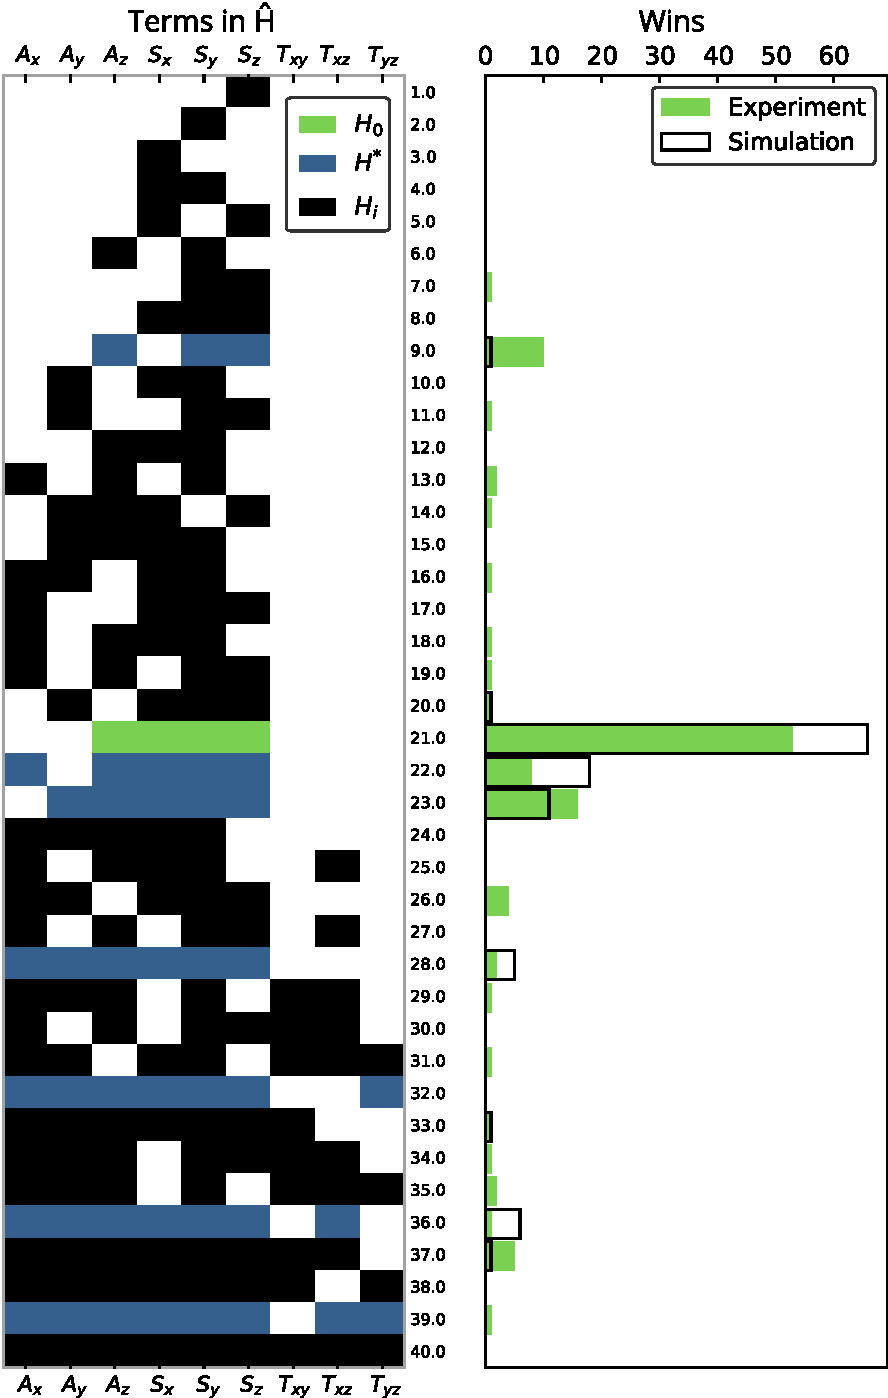
\includegraphics[width=0.6\textwidth]{experimental_study/figures/model_composition.pdf}
    \end{center}
    \caption[
        Models considered by QMLA for simulated/experimental nitrogen-vacancy centre data, and their win rates
    ]{
    \textbf{Left,} map of the various \gls{hamiltonian} terms included in each of the possible 40 candidate models explored by \gls{qmla}
    during any of the 100 \glspl{instance} on either simulated or experimental data.
    IDs of candidate models are on the vertical axis, and labels for the terms on the horizontal axis.
    The \gls{true model} $\hat{H}_0$ for the simulated case is highlighted in green and a subset of credible models in blue, 
    i.e. models which may reasonbaly be expected to describe the targeted \glsxtrlong+{nvc} from theoretical arguments.
    \textbf{Right,} number of wins for each of the candidate models out of $100$ independent \gls{qmla} \glspl{run}. 
    Cases adopting simulated data are shown by empty bars, with those using the experimental dataset shown by green bars.
    \figtableref
    } 
    \label{fig:nv_model_composition}
\end{figure}

Here we offer some further perspectives, 
    considering the \glspl{run} summarised in \cref{fig:exp_qmla_analysis}.
\cref{fig:nv_model_composition} first details all \glspl{model} considered in the 200 \glspl{instance} 
    comprising the experimental and simulated \gls{qmla} \glspl{run}, 
    as well as the  \gls{win rate}  of each model. 
This \gls{es} is designed to study a small subspace of the overall available space:
    only $40$ unique models are constructed. 
We highlight a number of \emph{credible} models which we deem especially valid approximations of the target system, 
    i.e. which contain the most viable approximations. 
\par 

\begin{figure}[t]
    \centering
    \begin{tabular}{@{}c@{}}
        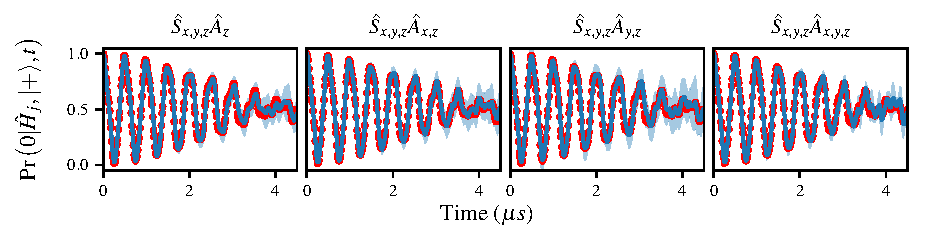
\includegraphics[scale=0.99]{experimental_study/figures/reproduced_dyamics_sim.pdf}
    \end{tabular}
    \\ \small \textbf{(a)} Simulated data
    \centering

    \begin{tabular}{@{}c@{}}
        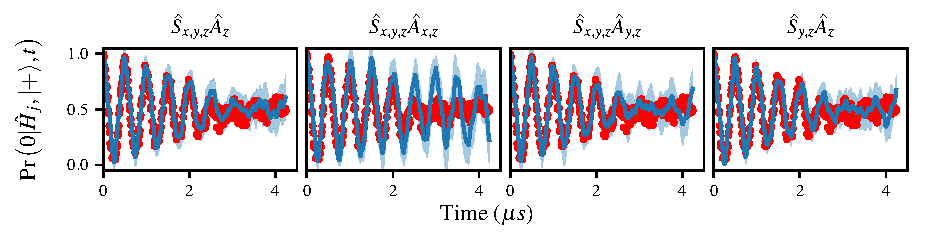
\includegraphics[scale=0.99]{experimental_study/figures/reproduced_dyamics_exp.pdf}
    \end{tabular}
    \\ \small \textbf{(b)} Experimental data

    \caption[Dynamics reproduced by QMLA champion models for simulated/experimental data]{
        Dynamics reproduced by various \gls{qmla} \glspl{champion model} for \textbf{(a)} simulated and \textbf{(b)} experimental data. 
        Likelihoods, $\Pr(0)$ are shown on $y$--axis with time on $x$--axis. 
        Red dots give the true dynamics of $\ho$, while the blue lines show the median reconstruction by $\hp$
        from all the \glspl{instance} where that model was deemed $\hp$, with light blue showing the $67\%$ confidence region.
        $\hp$ \ is listed on top of each plot; the number of \glspl{instance} won by each model can be read from \cref{table:win_rates_r_squareds}.
        \figtableref 
        }
    \label{fig:nv_model_dynamics}
    % in figure_development/nv_dynamics_reproduction.ipynb
\end{figure}

\cref{fig:nv_model_dynamics} shows the reproduction of dynamics of the top\footnotemark \ 
    four \glspl{model} from both simulated and experimental \glspl{run}. 
We see that each model faithfully captures the essential dynamics arising from the respective target systems;
    this alone is insufficient to conclude that the \gls{true model} has been identified, 
    but serves as a valuable \emph{sanity-check}, convincing us that the output of \gls{qmla} is at least a sensible 
    approximation of $\ho$, if not the absolute \gls{true model}.
\footnotetext{
    \emph{Top} models in the context of \gls{qmla} are those \glspl{model} within the \gls{run} with 
    the highest \glspl{win rate}, i.e. which won more \glspl{instance} than other candidates
    from the \gls{model space}.
}
\par 

The key insight promised by \gls{qmla} is to identfiy the interactions present in the studied system, 
    which in this case was the decoherence processes of an \gls{nvc}.
In \cref{fig:nv_learned_params} we show the number of times each of the terms permitted, 
    i.e. $\hat{t} \in \termset_{\textrm{NV}}$ from \cref{eqn:nv_terms},
    are included in the \gls{champion model},
    as well as the distribution of parameter estimates for those terms. 
From the simulated case, we see that those terms which are in $\ho$, i.e. $\hat{t} \in \termset_0$, are found in almost all instances.
Furthermore, while most instances find a \gls{champion model} which includes some erroneous term(s), 
    each $\hat{t} \notin \termset_0$ is found with less than a quarter of the frequency of those $\hat{t} \in \termset_0$.
Hence terms outside of $\termset_0$ may be reasonably ruled out in post-processing the \gls{qmla} results, 
    by manually considering the relative frequency with which each term is found. 
The inaccurate terms found most often are seen to have (almost) negligible parameters:
    in conjunction with domain expertise, users can determine whether the inclusion of these terms 
    are meaningful or simply artefacts of slight overfitting.
In the experimental \gls{run}, on the other hand, we see a similar gulf in frequency between some terms.
Namely, $\{ \hat{S}_x, \hat{S}_y, \hat{S}_z, \hat{A}_z \}$ are found in over $50$ \glspl{instance} \emph{more} than all other terms:
    we therefore conclude that those terms contribute most strongly to the \gls{nvc}'s decoherence process.
The resultant model, $\hat{S}_{xyz}\hat{A}_{z}$ is in agreement with theoretical expectations, 
    and shows that we can describe the intricate processes involved in decoherence through a relatively simple 
    \gls{hamiltonian}, proving that \gls{qmla} can perform an important role in aiding the understanding of quantum systems.  
\par 

\begin{figure}
    \thisfloatpagestyle{empty} % caption goes over page number so supressing it
    \centering
    \begin{tabular}{@{}c@{}}
        \centering
        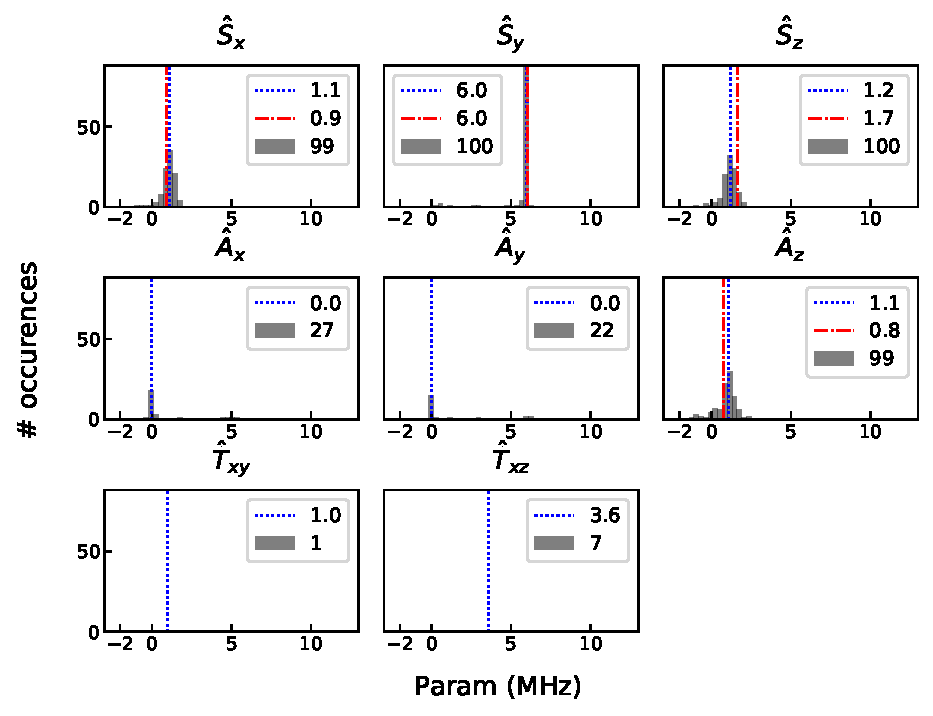
\includegraphics[width=0.7\textwidth]{experimental_study/figures/params_simulation.pdf}
    \end{tabular}
    \\ \small \textbf{(a)} Simluated QMLA instances. Red dotted lines show the true parameters.
    
    \centering
    \begin{tabular}{@{}c@{}}
        \centering
        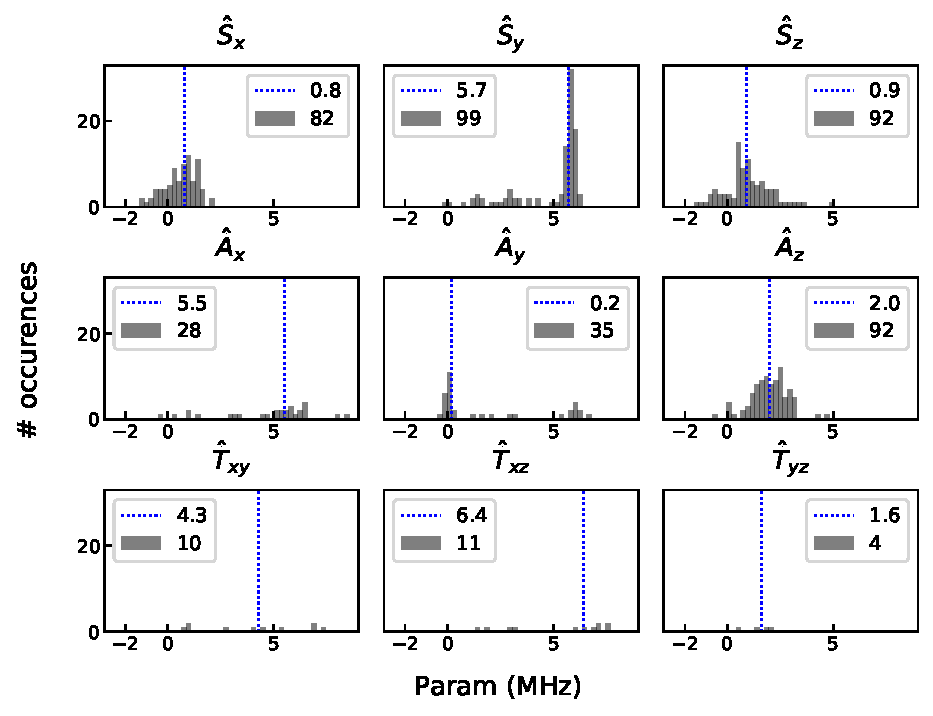
\includegraphics[width=0.7\textwidth]{experimental_study/figures/params_experimental.pdf}
    \end{tabular}
    \\
    \small \textbf{(b)} Experimental QMLA instances.
    \caption[
        Histograms for parameters learned by QMLA champion models on simulated and experimental data
    ]{
        Parameter values for terms found by \gls{qmla}. 
        For each term found within the \gls{champion model} of at least one \gls{instance} of \gls{qmla}, 
            a histogram is shown for the values of the term's associated parameter.
        The terms are listed along the top of each subplot with results for (\textbf{a}) simulated  and (\textbf{b}) experimental data. 
        Blue dotted lines indicate the median for that parameter, while red dotted lines give the true parameter in the simulated case. 
        Grey blocks show the number of champion models which found the parameter to have that value,
        and the number listed in the legend reports the total number of \glspl{champion model} which contained that term.
        \figtableref
    }
    \label{fig:nv_learned_params}
\end{figure}


\subsection{Finite size effects}
The case examined in this chapter is fundamentally limited by the nature of the approximation: 
    by assigning a closed Hamiltonian to the \gls{nvc}, 
    we may never retrieve a complete description of the system. 
Closed, conservative  dynamical systems -- with a finite spectrum of permissible states -- 
    will return to their initial state after some finite time, 
    according to the Poincar\'e recurrence theorem \cite{breuer2002theory}.
For quantum systems, then, the Poincar\'e recurrence times $\{t_R\}$ correspond to the times at which 
    the \emph{global} system's state, $\ket{\psi_g}$, returns to its starting state, 
    $\absval{\braket{\psi_{\rm{g}}(t_R) | \psi_{\rm{g}}(0)}}^2 \approx 1$
    \cite{gentile2020Operating}.
Such a system is therefore expected to exhibit \emph{revivals}; 
    in the context of quantum many-body systems,
    this is where the system \emph{rephases} some time after it had dephased. 
These revivals are not necessarily physical, 
    but rather an artefact of the approximation:
    realistic systems are seen to decohere completely after some decoherence time
    without revivals, i.e. \emph{irreversible decoherence}. 
The Poincar\'e recurrence time scales polynomially with the number of degrees of freedom, $n$,
    within the closed system:  $t_R \sim n!$. 
That is, even though the system of many interacting components \emph{will} rephase, 
    the time required to do so may be greater than the age of the universe \cite{schlosshauer2005decoherence}. 
Conversely, in our simplistic two-qubit model, the spectrum of eigenenergies is artifically restricted, 
    and so revivals will appear unrealistically quickly. 
\par 
\cref{fig:predicted_revivals} shows the predicted revivals of $\hp = \hat{S}_{x,y,z}\hat{A}_z$, 
    the model found by \gls{qmla} to describe the \gls{nvc} in the above analysis. 
The predicted revivals are unlikely to correspond to further experimental data; 
    we can see intuitively that the system had decohered completely and irreversibly 
    after $\SI{4.2}{\micro\second}$.
When modelling such systems in practice, these revivals are often suppressed by a 
    time-dependent damping $e^{-\Gamma t}$, with $\Gamma$ determined phenomononoligcally,
    in order to yield the irreversible decoherence observed in real experimental systems,
    including the one used throughout this chapter. 
Here our aim was to model the interactions of the \gls{nvc} spin with its nearest environmental qubit,
    which would be undermined by including such a drastic time-dependent effect:
    we omit this factor in this work, 
    however it will prove important to account for this behaviour in future applications of \gls{qmla} to open systems.     

\begin{figure}
    \begin{center}
        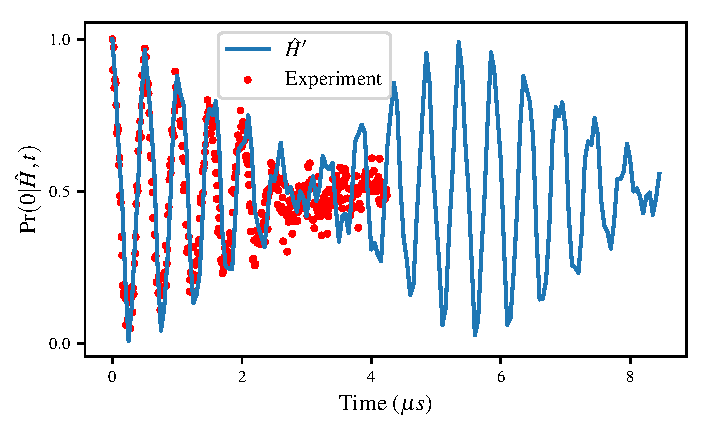
\includegraphics{experimental_study/figures/predicted_revivals.pdf}        
    \end{center}
    \caption[Predicted revivals of QMLA champion model]{
        Predicted revivals of \gls{qmla} \gls{champion model}, $\hp$ (blue), 
        against the experimental data (red). 
    }
    \label{fig:predicted_revivals}
\end{figure}

Invoking a finite-size bath to approximate the genuine open-system nature of the \gls{nvc} 
    permits us to examine the interaction of the spin with few neighbours, 
    sufficient to characterise the domainant decoherence processes of a system, as we have done in this chapter.
However, the approximation can not capture all of the spin's interactions, 
    so we are motivated to consider models involving more nuclei, 
    and ultimately models of open quantum system. 
In \cref{chapter:many_qubits} we consider a similar \gls{nvc} setup in simulation, 
    to explore \gls{qmla}'s capability while relaxing the effect of the finite size bath,
    and we note in \cref{chapter:outlook} that in order for \gls{qmla} to prove useful 
    in characterisation genuine quantum systems, we must incorporate complete open system models. 

\subsection{Outlook}
We have thus characterised the interactions which dominate the decoherence process for a given \gls{nvc}. 
In doing so, we identified not only the terms present, but also the strength (i.e. parameters) of those terms. 
Automated characterisation of quantum systems will be essential in the development of quantum technologies, 
    whether for calibration of controlled devices, or alignment of experimental systems for optimal results. 
While this demonstration must be understood in the context of its limitations, 
    e.g. the restricted basis studied, and the constrained \gls{model space} searched, 
    it represents a crucial proof of principle that \gls{qmla} is applicable to the task 
    of automated quantum system characterisation. 
In the next chapter, we extend \gls{qmla} in simulation, to overcome some of the limitations mentioned here. 
